\documentclass[12pt, a4paper]{report}

\usepackage{fontspec}
\IfFontExistsTF{Times New Roman}
  {\setmainfont{Times New Roman}}
  {\setmainfont{TeX Gyre Termes}}

\usepackage{polyglossia}
\setdefaultlanguage{english}
\setotherlanguage{romanian}

\usepackage{fvextra}
\usepackage{csquotes}
\usepackage[
    maxbibnames=3,
    minbibnames=1,
    giveninits=true,
    doi=false,
    isbn=false,
    sorting=none
]{biblatex}
\addbibresource{bibliography.bib}
\AtEveryBibitem{%
  \clearfield{url}%
  \clearfield{urldate}%
}
\renewbibmacro*{url+urldate}{}

\usepackage{setspace}
\onehalfspacing

\usepackage[margin=2.5cm]{geometry}
\usepackage{graphicx}
\graphicspath{{./images/}{../out/figures/}}
\usepackage{float}
\usepackage{listings}
\usepackage{minted}
\usepackage{array}
\usepackage{booktabs}
\usepackage{tikz}
\usetikzlibrary{arrows.meta,positioning}
\usepackage[
    colorlinks,
    linkcolor={black},
    menucolor={black},
    citecolor={black},
    urlcolor={blue}
]{hyperref}

\usepackage{amsmath}
\usepackage{mathtools}

\setlength{\textfloatsep}{10pt plus 2pt minus 2pt}
\setlength{\floatsep}{8pt plus 2pt minus 2pt}
\setlength{\intextsep}{8pt plus 2pt minus 2pt}
\setlength{\abovecaptionskip}{4pt}
\setlength{\belowcaptionskip}{0pt}

\newenvironment{abstractpage}
  {\cleardoublepage\vspace*{\fill}\thispagestyle{empty}}
  {\vfill\cleardoublepage}
\renewenvironment{abstract}[1]
  {\bigskip\selectlanguage{#1}%
   \begin{center}\bfseries\abstractname\end{center}}
  {\par\bigskip}

\usepackage{fancyhdr}

\fancypagestyle{front}{
  \fancyhf{}
  \renewcommand{\headrulewidth}{0pt}
  \cfoot{}
}

\fancypagestyle{main}{
  \fancyhf{}
  \renewcommand\headrulewidth{0pt}
  \fancyhead[C]{}
  \fancyfoot[C]{\thepage}
}

\setcounter{tocdepth}{2}
\setcounter{secnumdepth}{2}

\title{Inlining Compiler Optimization\\Through Machine Learning Techniques}
\author{Ingrid-Adriana Corobană}

\makeatletter

\begin{document}

\cleardoublepage
\pagestyle{front}
\let\ps@plain\ps@front
\pagenumbering{gobble}

\begin{titlepage}

\newgeometry{left=2cm,right=2cm,bottom=1cm}

\begin{figure}[!htb]
    \centering
    \begin{minipage}{0.2\textwidth}
        
\includegraphics[width=\linewidth]{logo-ub.png}
    \end{minipage}
    \begin{minipage}{0.5\textwidth}
        \large
        \vspace{0.2cm}
        \begin{center}
            \textbf{UNIVERSITY OF BUCHAREST}
        \end{center}
        \vspace{0.3cm}
        \begin{center}
            \textbf{
                FACULTY OF MATHEMATICS\\
                AND COMPUTER SCIENCE
            }
        \end{center}
    \end{minipage}
    \begin{minipage}{0.2\textwidth}
        
\includegraphics[width=\linewidth]{logo-fmi.png}
    \end{minipage}
\end{figure}

\begin{center}
\textbf{COMPUTER SCIENCE PROGRAM}
\end{center}

\vspace{1cm}

\begin{center}
\Large \textbf{Bachelor's Thesis}
\end{center}

\begin{center}
\huge \textbf{\MakeUppercase{\@title}}
\end{center}

\vspace{3cm}

\begin{center}
\large \textbf{Graduate \\ \@author}
\end{center}

\vspace{0.25cm}

\begin{center}
\large \textbf{Scientific Advisor \\ Prof. Dr. Cristian Rusu}
\end{center}

\vspace{2cm}

\begin{center}
\Large \textbf{Bucharest, 2026}
\end{center}

\end{titlepage}

\restoregeometry

\cleardoublepage
\pagenumbering{roman}

\begin{abstractpage}
\begin{abstract}{english}
The research area of compiler optimization continues to be relevant in
computer science because software is expected to stay compact and efficient
across different hardware environments while still meeting increasing
performance requirements. Even though compile-time inlining is a fundamental
optimization, choosing which call sites should be inlined remains difficult.
One local choice can change the following call graph and therefore the
optimization opportunities that later passes can still use. As a result,
inlining can either decrease or increase the size of the generated intermediate
representation and of the final binary.

In this work, the inlining problem is framed as an offline policy-learning
problem. For the implementation, C and C++ source files are collected from a
small DCMTK snapshot and from a varied public-source supplement, while
deterministic synthetic modules are added to extend the dataset with
controlled inlining cases. The files pass through the Clang frontend with the
inlining option turned off, in order to generate LLVM IR modules. Information
extracted from individual call sites is translated into feature vectors that
contain caller, callee, call-site, and call-graph information.

Multiple heuristics with a teacher role are used. Each module passes through
this heuristic set in order to determine which one minimizes rewritten IR size
best for that module. The selected heuristic's call-site choices become the
dataset for a supervised learning strategy, in which student models learn to
imitate teacher trajectories through behavior cloning. The students'
predictions are then integrated back into LLVM IR through call-site-level
rewrites. The reported run
compiles 163 C/C++ sources, evaluates 150 LLVM modules with local call sites,
and extracts 10394 call-site samples. On the held-out split, the
selected-teacher reference reduces rewritten LLVM IR instruction count by
1.10\% relative to never-inline, while the best held-out student reaches a
0.61\% reduction. These results do not outperform LLVM's production
\texttt{-Oz} pipeline, but they give insight into the possibility of treating
compile-time inlining decisions as machine-learning policy problems, not only
as fixed classical heuristics.
\end{abstract}
\end{abstractpage}

\begin{abstractpage}
\begin{abstract}{romanian}
Optimizarea compilatoarelor rămâne o ramură de cercetare importantă în
informatică, deoarece tehnologia evoluează într-o direcție în care aplicațiile
trebuie să fie compacte, rapide și eficiente pe platforme hardware diferite,
ținând în același timp pasul cu cerințele de performanță ale industriei. Deși
decizia de inlining la compilare reprezintă o optimizare fundamentală, alegerea
call site-urilor care trebuie înlocuite prin inlining rămâne complicată,
deoarece o decizie locală poate schimba graful de apeluri viitor, precum și
posibilitățile de optimizare pe care compilatorul le mai poate folosi ulterior.
Aceasta poate duce la creșterea sau scăderea dimensiunii reprezentării
intermediare generate și a dimensiunii binarului final.

În această lucrare, problema inlining-ului este formulată într-o manieră de
învățare offline. Pentru implementare, fișiere C și C++ sunt colectate dintr-un
snapshot DCMTK, din surse generate sintetic și dintr-un supliment variat de
surse publice selectate după compilare și filtrare după relevanța pentru
inlining. Fișierele trec prin frontend-ul Clang, cu inlining-ul dezactivat,
pentru a obține module LLVM IR. Informațiile extrase la nivel de call site sunt
transformate în vectori de trăsături care includ informații despre caller,
callee, call site și graful de apeluri.

Sunt folosite multiple euristici cu rol de profesor. Fiecare modul este evaluat
de fiecare astfel de euristică, cu scopul de a determina care dintre ele
minimizează cel mai bine dimensiunea LLVM IR rescrisă pentru modulul respectiv.
Alegerile euristicii selectate la nivel de call site devin un set de antrenare
pentru o strategie de învățare supervizată, în care modelele student învață să
imite traiectoriile profesorilor prin behavior cloning. Predicțiile studenților
sunt ulterior integrate înapoi în LLVM IR prin rescrieri la nivel de call site.
Rularea raportată compilează 163 de surse C/C++, evaluează 150 de module LLVM
cu call site-uri locale și extrage 10394 de exemple la nivel de call site. Pe
split-ul held-out, referința selected-teacher reduce numărul de instrucțiuni
LLVM IR rescrise cu 1.10\% față de never-inline, iar cel mai bun student ajunge
la o reducere de 0.61\%. Rezultatele nu depășesc pipeline-ul de producție LLVM
\texttt{-Oz}, dar demonstrează un workflow reproductibil de învățare offline
pentru experimente cu politici de inlining la nivel de call site.
\end{abstract}
\end{abstractpage}


\cleardoublepage
\begingroup
\small
\setstretch{1.10}
\setlength{\parskip}{0pt}
\tableofcontents
\endgroup

\cleardoublepage
\pagestyle{main}
\let\ps@plain\ps@main
\pagenumbering{arabic}


% =========================================================
% CHAPTER 1
% =========================================================

\chapter{Introduction}

Optimizing at compile time remains a current research topic, since compilers
must keep large builds deterministic enough while still producing compact, fast,
cross-platform code. As a result, many optimization decisions are still made
through heuristics: generalized rules that estimate whether a transformation is
worth applying. This thesis studies inlining as one concrete case where a local
decision can affect later passes, target behavior, and code size, so the best
choice is too situational to be captured well by one simple rule
\cite{godbolt2019optimizations,theodoridis2022optimal}.

Inlining represents a high-impact example of this problem. By substituting a
call site with the instructions corresponding to the called function, it can
remove call overhead and expose constant propagation, devirtualization,
dead-code elimination, and other later optimizations. Nonetheless, inlining can
also duplicate code and grow the final binary when the copied body is not useful
enough. Production compilers therefore use cost models and thresholds to
balance optimization opportunity against generated-code growth
\cite{godbolt2019optimizations,theodoridis2022optimal,mlgo}.

The purpose of this thesis is to analyze a smaller ML-guided alternative to
those manual baselines and to investigate whether a teacher-student model can
give useful results from static features and scenario-specialized teachers. The
implemented prototype evaluates several heuristics with a teacher role per
module, selects the best teacher trajectory under a rewritten-IR size objective,
and trains student policies to imitate the selected inline/no-inline decisions.
The setup follows the broad MLGO idea that compiler decisions can be driven by
features from the current context, while using offline imitation learning
instead of online reinforcement learning
\cite{milepostgcc,mlgo,llvmmlgo,bcmax}.

Function inlining is a useful case study because it requires both local and
global information. At call-site level, the compiler decides whether to replace
the call with the instructions of the called function, or to keep the function
call unchanged. At global level, this choice can change the program
representation: the caller can grow, the callee can become removable, the future
call graph can change, and later optimization opportunities may also change.
The prototype reproduces this setting in a
smaller environment: heuristics with a teacher role create inline/no-inline
trajectories, the best teacher per module is chosen by rewritten LLVM IR size,
and student classifiers learn the selected labels.

For evaluation, LLVM IR is modified using LLVM's \texttt{opt} tool. The number
of rewritten LLVM IR instructions becomes the primary metric used to assess the
student policies, while native object \texttt{.text} size is reported as a
secondary reference metric.

\section{Research Questions and Contributions}

\begin{table}[H]
\centering
{\small
\renewcommand{\arraystretch}{1.0}
\setlength{\tabcolsep}{3pt}
\begin{tabular}{|>{\raggedright\arraybackslash}p{0.055\textwidth}|
                >{\raggedright\arraybackslash}p{0.39\textwidth}|
                >{\raggedright\arraybackslash}p{0.455\textwidth}|}
\hline
ID & Research question & Thesis contribution \\
\hline
RQ1 & Can inlining be framed as offline imitation learning from heuristics with
a teacher role? &
Formalizes inlining as a binary call-site policy problem with teacher-role
heuristics, selected trajectories, and behavior cloning. \\
\hline
RQ2 & Can BC-Max-style selection produce call-site labels under a code-size
objective? &
Evaluates 16 teachers per module and builds selected-teacher labels for
supervised training. \\
\hline
RQ3 & Can simple students imitate selected teachers from static features? &
Implements the LLVM IR workflow for feature extraction, teacher design,
behavior cloning, rewriting, size measurement, and student training. \\
\hline
RQ4 & Do learned decisions reduce rewritten IR compared with never-inline? &
Applies predictions through cloned callees, \texttt{alwaysinline}, LLVM
\texttt{opt}, and held-out IR/native \texttt{.text} evaluation. \\
\hline
RQ5 & What gaps remain relative to production ML-guided inlining? &
Analyzes dataset scale, static rewrite approximation, teacher quality, and
missing full LLVM inliner integration. \\
\hline
\end{tabular}
}
\caption{Research questions and corresponding contributions.}
\label{tab:questions-contributions}
\end{table}

% =========================================================
% CHAPTER 2
% =========================================================

\chapter{Compiler Background}

\section{Compilation Pipeline}

Compilation transforms source code into representations that are easier for a
machine to execute. This thesis focuses on LLVM IR, since choosing whether to
inline affects the instruction count and can be inspected before
backend-dependent machine choices are made. A simplified LLVM-based pipeline is:

\begin{figure}[H]
\centering
\begin{tikzpicture}[
  node distance=0.42cm,
  stage/.style={
    draw,
    rounded corners,
    align=center,
    minimum width=4.55cm,
    minimum height=0.64cm,
    font=\small
  },
  arrow/.style={-{Latex[length=2mm]}, thick}
]
\node[stage] (source) {C++ source};
\node[stage, below=of source] (clang) {Clang frontend};
\node[stage, below=of clang] (ir) {LLVM IR (\texttt{.ll})};
\node[stage, below=of ir] (optir) {optimized LLVM IR};
\node[stage, below=of optir] (backend) {machine-specific backend};
\node[stage, below=of backend] (asm) {assembly text \\ optional visible output};
\node[stage, below=of asm] (obj) {object files \\ \texttt{.o}/\texttt{.obj}};
\node[stage, below=of obj] (link) {linker};
\node[stage, below=of link] (exe) {executable file};
\draw[arrow] (source) -- (clang);
\draw[arrow] (clang) -- (ir);
\draw[arrow] (ir) -- (optir);
\draw[arrow] (optir) -- (backend);
\draw[arrow] (backend) -- (asm);
\draw[arrow] (asm) -- (obj);
\draw[arrow] (obj) -- (link);
\draw[arrow] (link) -- (exe);
\end{tikzpicture}
\caption{Simplified LLVM-based compilation pipeline.}
\label{fig:llvm-pipeline}
\end{figure}

Through Clang, C or C++ source files are checked according to the language rules
and translated into LLVM IR. After IR optimization, the backend chooses target
instructions, maps virtual registers to real registers, and emits object code
\cite{cooper2011engineering,muchnick1997advanced}. LLVM IR is therefore useful
for this prototype: it is lower-level than source code but still abstract
enough to remain independent of the final object-file format.

\section{LLVM and LLVM IR}

LLVM is a compiler infrastructure project that includes optimizers, backend
tools, and libraries. LLVM IR does not represent the entirety of the LLVM
project, but only the intermediate representation used inside that
infrastructure \cite{llvmlangref,llvmpasses}. It contains virtual registers,
typed operations, branches, calls, and memory operations. These virtual
registers are placeholders later lowered by the backend during instruction
selection and register allocation.

\section{Static and Dynamic Measurements}

In this thesis, a distinction is made between static representations and
dynamic executions. A static call graph contains possible calls before one
concrete run is chosen, while a dynamic call graph keeps only calls that occur
for one input. Likewise, static code size is measured in an artifact such as a
native text section, while dynamic instruction count refers to executed
instructions
\cite{cooper2011engineering,godbolt2019optimizations}.

% =========================================================
% CHAPTER 3
% =========================================================

\chapter{Function Inlining}

Through inlining as a case study, various compiler optimization issues can be
highlighted. Although it seems simple at first glance, inlining is important
because one binary call-site decision can propagate through later compiler
passes. It removes a call boundary by
materializing the callee's operations inside the caller. The original call
instruction may disappear, the computational cost of dispatching through that
call can be avoided, and later passes can optimize values and control flow
across the merged code region
\cite{cooper2011engineering,muchnick1997advanced,godbolt2019optimizations}.

\section{Cases Where Inlining Helps}

The examples in this chapter are simplified examples written for this thesis.
Small arithmetic helper functions represent typical good inlining candidates:

\begin{figure}[H]
\centering
\begin{minipage}[t]{0.36\textwidth}
\begin{minted}[fontsize=\footnotesize,breaklines]{cpp}
int ab(int a, int b) {
    return a * b;
}
\end{minted}
\end{minipage}\hfill
\begin{minipage}[t]{0.55\textwidth}
\begin{minted}[fontsize=\footnotesize,breaklines]{cpp}
int sum_ab(int a, int b) {
    return a + b + ab(a, b);
}
\end{minted}
\end{minipage}
\caption{Small helper and caller before inlining.}
\label{fig:ab-sum-ab-example}
\end{figure}

Inlining \texttt{ab} removes a function call and replaces it with a small
multiplication expression. If this call belongs to a hot part of the program,
meaning a part that is executed frequently, saving the call overhead can be
beneficial.

Inlining is also useful in cases where constants can propagate. In the example
below, after inlining, the compiler can understand that \texttt{c} is always
zero in this call context, and this can lead to the simplification of the other
branches:

\begin{figure}[H]
\centering
\begin{minipage}[t]{0.49\textwidth}
\begin{minted}[fontsize=\footnotesize,breaklines]{cpp}
// before:
string light_color(int c, int i) {
    if (c == 0)
        return light_red(i);
    if (c == 1)
        return light_green(i);
    return light_blue(i);
}

string car_color(int i) {
    int f = i;
    return light_color(0, 2 + f);
}
\end{minted}
\end{minipage}\hfill
\begin{minipage}[t]{0.47\textwidth}
\begin{minted}[fontsize=\footnotesize,breaklines]{cpp}
// after:
string car_color(int i) {
    int f = i;
    return light_red(2 + f);
}
\end{minted}
\end{minipage}
\caption{Constant-propagation example before and after inlining.}
\label{fig:inline-constant-example}
\end{figure}

\section{Cases Where Inlining Hurts}

Recursive functions can lead to uncontrolled code expansion, and in such cases
inlining should usually be avoided:

\begin{figure}[H]
\centering
\begin{minipage}[t]{0.47\textwidth}
\begin{minted}[fontsize=\footnotesize,breaklines]{cpp}
int sum(int x) {
    if (x <= 0)
        return 0;
    return x + sum(x - 1);
}
\end{minted}
\end{minipage}\hfill
\begin{minipage}[t]{0.42\textwidth}
\begin{minted}[fontsize=\footnotesize,breaklines]{cpp}
// recursive inlining:
// exposes another recursive call
// repeated expansion
// needs recursion/growth checks
\end{minted}
\end{minipage}
\caption{Recursive call site and the reason it is usually rejected.}
\label{fig:recursive-inline-risk}
\end{figure}

In contrast with hot parts of a program, choosing to inline a rarely called
large function can be damaging:

\begin{figure}[H]
\centering
\begin{minipage}[t]{0.47\textwidth}
\begin{minted}[fontsize=\footnotesize,breaklines]{cpp}
void game_engine_reinit() {
    // large recovery path
}
\end{minted}
\end{minipage}\hfill
\begin{minipage}[t]{0.45\textwidth}
\begin{minted}[fontsize=\footnotesize,breaklines]{cpp}
void entry(bool error) {
    if (error)
        game_engine_reinit();
}
\end{minted}
\end{minipage}
\caption{Cold-path callee and caller: inlining the recovery function can grow
static code size and instruction-cache pressure with little hot-path benefit.}
\label{fig:cold-path-example}
\end{figure}

Another bad case appears when a large callee is copied at multiple call sites:

\begin{figure}[H]
\centering
\begin{minipage}[t]{0.49\textwidth}
\begin{minted}[fontsize=\footnotesize,breaklines]{cpp}
int get_info(int id) {
    int s = id;
    for (int i = 0; i < 1000; ++i)
        s = (s * 33) ^ i;
    return s;
}
\end{minted}
\end{minipage}\hfill
\begin{minipage}[t]{0.47\textwidth}
\begin{minted}[fontsize=\footnotesize,breaklines]{cpp}
void info_candidates() {
    cout << get_info(12) << endl;
    cout << get_info(133) << endl;
    cout << get_info(144) << endl;
    // can grow code unnecessarily
}
\end{minted}
\end{minipage}
\caption{Large callee copied at multiple call sites if inlined aggressively.}
\label{fig:get-info-example}
\end{figure}

% =========================================================
% CHAPTER 4
% =========================================================

\chapter{Problem Formulation}

Let \(P\) be a program or module, and let
\[
  C(P) = \{c_1,c_2,\ldots,c_n\}
\]
be the set of all call sites observed during the inlining pass. Call sites are the
locations of function calls, where a caller function invokes another function,
called the callee. For each call site \(c_i\), the compiler can extract
information from the call site and from the call graph in order to form a
feature vector:
\[
  x_i = \phi(c_i),
\]
where \(\phi\) is the feature-extraction function. In this thesis, the static
features include caller and callee shape, instruction and call counts,
constant-argument information, recursion information, and limited call-graph
context.

The possible action choice is binary:
\[
  A = \{0,1\}, \qquad 0 = \text{do not inline}, \qquad 1 = \text{inline}.
\]

A probabilistic policy assigns a score or probability to each action:
\[
  \pi_\theta(a \mid x)
\]
where \(\pi_\theta(a \mid x)\) denotes the likelihood of choosing action \(a\),
given feature vector \(x\). The deterministic inline/no-inline decision used
by the prototype is then
\[
  d_\theta(x) = \arg\max_{a \in A}\pi_\theta(a \mid x).
\]

Because of inlining, the problem is chronological and interdependent. If a
policy \(\pi\) is applied to a program \(P\), it creates the trajectory:
\[
  \tau_{\pi}(P)
  =
  ((x_1,a_1),(x_2,a_2),\ldots,(x_T,a_T)),
\]
where \(T\) is the number of inlining decisions made for that program. After
one call site is inlined, the caller may grow, the callee may become dead, and
later simplifications may appear. Local decisions are therefore not fully
independent \cite{mlgo,bcmax}.

The implementation uses a static offline approximation of this formulation: it
collects call sites from the initial LLVM IR, predicts labels, and applies
selected rewrites in one pass. It does not attempt online learning, where the
model would keep learning from new feedback during compilation. It also does
not update the call graph and recompute features after each individual rewrite,
as LLVM's online inliner could. Instead, the experiment trains from a fixed
dataset and applies a fixed batch of decisions to each module.

The objective is to minimize generated code size. In the prototype, the main
way of measuring how good a policy is uses the final rewritten LLVM IR
instruction count:
\[
  \mathrm{Size}_{IR}(P,\pi), \qquad
  R(P,\pi) = -\mathrm{Size}_{IR}(P,\pi).
\]
A lower value is better; equivalently, the reward is written as negative size.

Let
\[
  \mathcal{H} = \{h_0,h_1,\ldots,h_k\}, \qquad
  h^\star(P_j)=
  \arg\min_{h_i \in \mathcal{H}} \mathrm{Size}_{IR}(P_j,h_i)
\]
be the set of heuristics with a teacher role and the selected teacher for
module \(P_j\). Each heuristic \(h_i\) maps call-site-level information to
inline/no-inline choices.

The trajectory corresponding to the selected teacher is then added to the
supervised learning data:
\[
  \mathcal{D}
  =
  \bigcup_j
  \{(x_{j,t}, a^{\star}_{j,t})\}_{t=1}^{T_j},
\]
where \(a^{\star}_{j,t}\) is the action taken by the selected teacher
\(h^\star(P_j)\) for feature vector \(x_{j,t}\).

A student model \(\pi_\theta\) is trained through behavior cloning. In the
ideal case, the student minimizes disagreement between its own choices and the
actions chosen by the selected teacher:
\[
  \min_{\theta}\sum_{(x,a)\in \mathcal{D}}
  \mathbf{1}[\pi_\theta(x) \neq a], \qquad
  \mathcal{L}(\theta)
  =
  -\sum_{(x,a)\in\mathcal{D}}\log \pi_\theta(a \mid x).
\]
In practice, the implementation trains standard classifiers; for probabilistic
models, the second expression is the binary cross-entropy.

After training, the student can be treated as a new heuristic. At each call
site, it receives the current feature vector and predicts whether to inline:
\[
  \hat{a} = \arg\max_{a\in\{0,1\}} \pi_\theta(a \mid x).
\]
The predicted decisions are then applied in the LLVM IR rewrite stage, which is
necessary in order to obtain the final rewritten instruction count used as the
metric.

% =========================================================
% CHAPTER 5
% =========================================================

\chapter{Related Work}

\section{Classical and Empirical Views of Inlining}

Inlining has been studied long before modern learned compiler policies. A
classical inliner estimates the benefit of removing a call and enabling later
optimizations, then compares it with the risk of code growth. Theodoridis,
Grosser, and Su show that optimal inlining remains nontrivial because decisions
interact with call chains, code size, and later passes
\cite{theodoridis2022optimal}. Godbolt's compiler-optimization examples give
the same practical motivation: inlining can expose constants, unreachable
branches, and other caller-specific information hidden behind the call boundary
\cite{godbolt2019optimizations,godbolt2025inlining}.

\section{Autotuning and Pre-MLGO Compiler Learning}

Before MLGO, several works already treated compiler optimization as empirical
search or learning. MILEPOST GCC uses program features to select optimization
choices instead of relying only on one fixed optimization level
\cite{milepostgcc}. Its relevance here is methodological: it shows that
compiler heuristics can be learned from empirical data, although it addresses
broader optimization selection rather than call-site-level inlining.

Inlining-specific autotuning also predates the current MLGO line of work.
Cavazos and O'Boyle study automatic tuning of inlining heuristics, showing that
parameters of an inliner can be adjusted empirically instead of being chosen
entirely by hand \cite{cavazos2005automatic}. This is close to the problem in
this thesis because it focuses on inlining, but the emphasis is different. The
goal there is to tune a heuristic; the goal here is to learn a policy from
selected teacher trajectories. In other words, autotuning searches for better
heuristic parameters, while behavior cloning tries to learn a decision rule
over call-site features.

More recently, MLGOPerf extends ML-guided inlining toward performance rather
than only code size \cite{mlgoperf}. Runtime can be more directly useful for
deployed software, but it introduces measurement noise and dependence on
hardware and inputs. This thesis therefore uses LLVM IR instruction count as
its primary low-compute metric and reports native \texttt{.text} size as a
secondary metric.

\section{MLGO}

MLGO represents a starting point and a primary example of how learned
decision-making policies can be integrated into LLVM optimization heuristics
\cite{mlgo,llvmmlgo}. For inlining, the state is represented by current
call-graph and call-site features, the action is inline or no-inline, and the
reward is a final compiled-program improvement, often native code-size
reduction for inlining-for-size. Because the full call graph is expensive to
use directly, the compiler exposes a feature vector about the caller, callee,
call site, and global graph. The original MLGO inlining setup uses
policy-gradient training with a delayed reward, which is powerful but expensive
because each environment interaction requires compilation
\cite{mlgo}.

\section{Offline Imitation Learning and BC-Max}

Marinov, Agarwal, and Trofin propose a cheaper alternative to online
reinforcement learning through offline imitation learning from multiple
baselines \cite{bcmax}. In the inlining setting, let
\[
  \mathcal{H} = \{h_0, h_1, \ldots, h_n\}
\]
be the set of heuristics with a teacher role, where \(P_i\) is one module and
\(\mathrm{Size}_{IR}(P_i, h)\) is the rewritten LLVM IR instruction count
obtained when teacher \(h\) is applied to \(P_i\).

For each module, the best teacher is the one with the smallest rewritten IR
size:
\[
  h^\star_i = \arg\min_{h \in \mathcal{H}} \mathrm{Size}_{IR}(P_i, h).
\]
The selected-teacher trajectory is then:
\[
  \tau_i = \{(s_1, h^\star_i(s_1)), \ldots, (s_m, h^\star_i(s_m))\}.
\]
Here, \(s_t\) is the feature vector for the \(t\)-th call site. The union of
these trajectories becomes a supervised dataset, and a student policy
\(h_{n+1}\) learns selected-teacher labels rather than exploring by repeated
compilation.

Teacher labels are not universal labels for isolated call sites. Rather, they
represent what the selected teacher thinks is best in that setting. Since
decisions are not only call-site-dependent, but also context-dependent, similar
local call sites may receive different labels in different modules if the best
module-level teacher is different. This creates possible label conflicts in the
behavior-cloning dataset. It is also one reason why the final result must be
measured after applying the predicted rewrites, not only by checking label
agreement.

\section{Positioning Against Prior Work}

Table~\ref{tab:related-work-summary} summarizes how the prototype borrows the
policy-learning view from MLGO and BC-Max while remaining smaller and more
inspectable than production compiler infrastructure.

\begin{table}[H]
\centering
\small
\setlength{\tabcolsep}{4.5pt}
\renewcommand{\arraystretch}{1.14}
\begin{tabular}{|>{\raggedright\arraybackslash}p{2.75cm}|
                >{\raggedright\arraybackslash}p{3.35cm}|
                >{\raggedright\arraybackslash}p{3.15cm}|
                >{\raggedright\arraybackslash}p{4.25cm}|}
\hline
Work & Main idea & Evaluation focus & Relation to this thesis \\
\hline
Cavazos and O'Boyle \cite{cavazos2005automatic}
& empirical tuning of inliner parameters
& benchmark performance
& early evidence that inlining choices can be optimized empirically \\
\hline
MILEPOST GCC \cite{milepostgcc}
& program-feature-based optimization selection
& empirical benchmark performance
& broad compiler ML rather than call-site-level inlining \\
\hline
MLGO \cite{mlgo,llvmmlgo}
& learned policies integrated inside LLVM
& code size and performance on large corpora
& main learned-heuristic reference, not reproduced here \\
\hline
BC-Max \cite{bcmax}
& offline imitation learning from multiple baselines
& final objective value
& closest template for teacher selection and behavior cloning \\
\hline
Theodoridis et al. \cite{theodoridis2022optimal}
& autotuned search for high-reduction inlining-for-size decisions
& native binary size on SPEC2017, LLVM, and SQLite
& motivates code-size evaluation and stronger baselines \\
\hline
This thesis
& BC-Max-style supervised pipeline over static call-site features
& rewritten IR and native text-section reference
& inspectable offline pipeline for call-site-level policy experiments \\
\hline
\end{tabular}
\renewcommand{\arraystretch}{1}
\caption{Related-work positioning for ML-guided and empirical inlining optimization.}
\label{tab:related-work-summary}
\end{table}

% =========================================================
% CHAPTER 6
% =========================================================

\chapter{Methodology}

The experimental pipeline follows Figure~\ref{fig:llvm-pipeline} until LLVM IR
is produced, and the main goal is to output LLVM IR that is as small as
possible. From that point, the prototype extracts call-site features, evaluates
teachers, selects the best teacher per module, trains student classifiers, and
applies predicted decisions through an \texttt{opt}-based IR rewrite. Source
collection, IR generation, teacher choice, student training, rewriting, and
measurement remain visible in the repository.

The C/C++ sources include a small DCMTK snapshot\footnote{DCMTK source
repository: \url{https://github.com/DCMTK/dcmtk}.}, 70 deterministic generated
modules, and 76 public-source files selected after compilation and
inlining-relevance filtering. The generator samples a \(4^6=4096\)
configuration space covering callee profiles, call mixes, argument patterns,
helper-body shapes, driver shapes, and explicit size profiles. This creates
tiny helpers, branch-heavy helpers, medium arithmetic helpers, large shared
callees, recursive calls, variable operands, and constant operands. The 70
generated modules contain 1120 driver call sites, giving the teachers both
inline and no-inline cases while broader benchmark transfer remains future
work.

The public-source supplement is kept only when a file compiles to LLVM IR,
exposes at least one local call site, and produces a measurable
teacher-selection artifact through the rewrite pipeline. These filters are
applied before student training and are part of dataset construction. The
implemented features are a smaller local approximation of the public MLGO
inlining schema: caller, callee, call-site, and module graph information, with
instruction counts, call counts, constant arguments, and recursion indicators
added for interpretability.

\begin{table}[H]
\centering
{\small
\renewcommand{\arraystretch}{1.08}
\setlength{\tabcolsep}{3pt}
\begin{tabular}{|>{\raggedright\arraybackslash}p{0.17\textwidth}|
                >{\raggedright\arraybackslash}p{0.35\textwidth}|
                >{\raggedright\arraybackslash}p{0.10\textwidth}|
                >{\raggedright\arraybackslash}p{0.27\textwidth}|}
\hline
Feature group & Implemented fields & Type & What the values indicate \\
\hline
Caller shape & caller-prefixed counts: basic blocks, conditional blocks,
users, IR instructions, and call instructions & numeric & size and branching
of the function that receives the inlined body; large or call-heavy callers may
already be expensive to grow \\
\hline
Callee shape & callee-prefixed counts: basic blocks, conditional blocks,
users, IR instructions, and call instructions & numeric & estimated body copied
by inlining, plus whether the callee has few users and may become removable
after all useful calls are inlined \\
\hline
Call-site context & \texttt{callsite\_height}, \texttt{cost\_estimate}, and
number of constant parameters & numeric & local decision context:
approximate graph depth, proxy inline cost, and constants that may enable
simplification after the callee body is copied into the caller \\
\hline
Module graph & module edge count and node count & numeric & rough module-level
density, used to distinguish sparse files from call-heavy modules where one
decision can interact with many nearby calls \\
\hline
Safety signal & recursive-call indicator & binary & marks recursive expansion
patterns, where repeated inlining can grow code unnecessarily \\
\hline
\end{tabular}
}
\caption{Grouped feature schema used by all teachers and students. The complete
ordered feature list is fixed in \texttt{scripts/data.py}.}
\label{tab:feature-schema}
\end{table}

\section{Dataset Summary}

The current prototype uses a DCMTK-based source snapshot, generated modules,
and a public-source supplement in order to test the offline
imitation-learning pipeline on a nontrivial number of call sites.

\begin{table}[H]
\centering
\begin{minipage}[t]{0.54\textwidth}
\centering
{\small
\setlength{\tabcolsep}{2pt}
\begin{tabular}{|p{0.53\linewidth}|p{0.39\linewidth}|}
\hline
Quantity & Value \\
\hline
Source mix & DCMTK, generated, 76 public files \\
\hline
Candidate C/C++ files & 164 \\
\hline
Compiled C/C++ files & 163 \\
\hline
Modules with local call sites & 150 \\
\hline
Extracted call sites & 10394 \\
\hline
Train samples & 9009 \\
\hline
Hold-out samples / modules & 1385 / 26 \\
\hline
Teacher policies / students & 16 / 7 \\
\hline
Primary metric & rewritten IR instructions \\
\hline
Secondary metric & native \texttt{.text} size \\
\hline
\end{tabular}
}
\end{minipage}\hfill
\begin{minipage}[t]{0.43\textwidth}
\centering
{\small
\begin{tabular}{|l|r|r|}
\hline
Source group & \shortstack{Teacher\\IR red.} &
\shortstack{Student\\IR red.} \\
\hline
Generated & 8.76\% & 2.75\% \\
\hline
Real source & 1.22\% & 1.08\% \\
\hline
All modules & 1.66\% & 1.18\% \\
\hline
\end{tabular}
}
\end{minipage}
\caption{Dataset summary and source-group IR reduction. ``Teacher'' means the
selected-teacher reference; ``Student'' means the best full-set student
\texttt{conservative\_forest}. The most frequent selected teachers are
\texttt{small\_callee} on generated modules and \texttt{greedy\_ir\_size} on
real-source modules.}
\label{tab:source-group-reduction}
\end{table}

At call-site level, 9128 of the 10394 examples come from public source files.
The train/test split is performed by module rather than by individual call
site, so all call sites from one module stay on the same side of the split.
This avoids testing on contexts that are nearly duplicated from the same caller,
callee, or call graph.

\begin{table}[H]
\centering
{\footnotesize
\setlength{\tabcolsep}{3pt}
\begin{tabular}{|p{0.18\textwidth}|r|r|p{0.18\textwidth}|p{0.27\textwidth}|}
\hline
Candidate group & Files & Compiled & Included & Reason \\
\hline
DCMTK snapshot & 18 & 17 & yes & source-level local call sites \\
\hline
Generated modules & 70 & 70 & yes & controlled inlining and no-inlining
patterns \\
\hline
Public sources & 76 & 76 & yes & compiled C/C++ files with local call-site
signal \\
\hline
\end{tabular}
}
\caption{Dataset accounting. Filtering is applied before student training and
keeps source-level modules with local call sites relevant to the rewritten-IR
objective.}
\label{tab:dataset-accounting}
\end{table}

\section{Teacher-Role Heuristics}

The local set of teacher-role heuristics is intentionally simple and
inspectable. The teachers use deterministic rules starting from the same
call-site-level feature vector. Let \(s\) be callee size, \(u\) callee users,
\(b\) branch count, \(k\) constant arguments, and \(r\) a recursion flag. Most
rules use the following general shape:
\[
  \text{inline if } B(x)-C(x)>0,\quad
  B(x)\approx 2k+\mathbf{1}_{u=1}+\text{depth signal},\quad
  C(x)\approx s+b+\text{nested calls}+r .
\]
The exact thresholds are fixed in \texttt{teach.py}; the table gives the
readable form of each rule. The exception is \texttt{greedy\_ir\_size}, whose
labels are produced by measured rewrites in \texttt{rewrite.py}. Therefore,
most teacher-role heuristics are cheap proxy policies, while the greedy
heuristic is slower because it actually tests candidate rewrites.

\begin{table}[H]
\centering
{\footnotesize
\setlength{\tabcolsep}{3pt}
\begin{tabular}{|p{0.25\textwidth}|p{0.65\textwidth}|}
\hline
Teacher & Short rule \\
\hline
\texttt{never\_inline} & Conservative baseline: never inline. \\
\hline
\texttt{small\_callee} & Inline if \(s\) is small and \(r=0\). \\
\hline
\texttt{single\_caller} & Inline if \(u=1\) and the callee is not large; the
standalone helper may disappear after cleanup. \\
\hline
\texttt{constant\_argument} & Inline if \(k>0\), so caller-known constants may
remove branches or simplify expressions. \\
\hline
\texttt{cost\_budget}, \texttt{growth\_budget} & Inline if estimated growth
\(G\approx s\max(1,u)+b+\text{nested calls}\) stays under a budget. \\
\hline
\texttt{loop\_averse}, \texttt{hot\_leaf} & Prefer leaf-like callees; reject
large, branchy, or call-heavy callees. \\
\hline
\texttt{balanced\_score}, \texttt{llvm\_like\_size},
\texttt{benefit\_cost\_ratio} & Inline if \(B(x)/\max(1,C(x))\) passes a
threshold. \\
\hline
\texttt{aggressive\_speed} & Accept more small and medium calls, while still
rejecting recursive or clearly large cases. \\
\hline
\texttt{ml\_linear\_score} & Inline if \(w\cdot x+\beta>0\), using fixed
hand-written weights rather than training. \\
\hline
\texttt{bandit\_ucb\_proxy} & Inline if \(\widehat{g}(x)+\alpha/\sqrt{1+u}>0\):
estimated gain plus a small uncertainty bonus. \\
\hline
\texttt{rl\_value\_proxy} & Inline if immediate simplification plus future
call-graph value exceeds growth penalty. \\
\hline
\texttt{greedy\_ir\_size} & Measured teacher: order plausible non-recursive
candidates, try candidate rewrites, and keep a candidate only when the actual
rewritten IR instruction count decreases. \\
\hline
\end{tabular}%
}
\caption{Teacher policies as readable decision rules.}
\label{tab:teacher-policies-readable}
\end{table}

The ML-, bandit-, and RL-inspired teachers are approximations rather than
actually trained teachers. The measured greedy teacher is more expensive
because it orders plausible candidates from static features, then uses the same
clone-and-\texttt{alwaysinline} rewrite path as evaluation and keeps only
locally improving rewrites. This distinction matters because the student does
not learn from a single oracle; it learns from the teacher that behaves best
for each module under the rewritten-IR objective.

The main reported run uses one offline teacher-selection round: teachers are
evaluated, one teacher trajectory is selected per module, and students imitate
those selected labels. Chapter~8 also reports a small three-round check in
which the best learned student is fed back as another measured candidate
policy.

% =========================================================
% CHAPTER 7
% =========================================================

\chapter{Implementation}

The main pipeline and implementation are located in the repository root. The
implementation generates synthetic modules, uses
compilation stages to reach LLVM IR, extracts call-site features, evaluates
teacher policies, trains students from the best-performing teachers, rewrites
selected call sites, and writes artifacts that can be inspected. The source
repository is available at:
\begin{center}
\small\url{https://github.com/dirgnic/optimizingInlining}
\end{center}

\section{Repository Structure and Execution}

The scripts cover generation, feature extraction, teacher selection, student
training, rewriting, and figure generation. After cloning the repository, the
full pipeline can be run from the repository root with
\texttt{python3 scripts/run.py all}. A short inspection run is available as
\texttt{python3 scripts/run.py demo}; it compiles a few generated modules,
prints the extracted call-site order and inline/keep decisions, and writes
before/after demo IR under \texttt{out/demo/rewritten/}. The reported numbers come from
deterministic source generation, a small number of DCMTK files, and a fixed
module-level train/test split, with artifacts written under \texttt{out/}.

The default execution path is organized as shown in
Table~\ref{tab:pipeline-scripts}. Only scripts used by the reported run are
listed here.

\begin{table}[H]
\centering
{\small
\begin{tabular}{|p{0.07\textwidth}|p{0.24\textwidth}|p{0.58\textwidth}|}
\hline
Step & Script & Role \\
\hline
0 & \texttt{data.py} & defines shared directories, feature names, and
call-site data structures. \\
\hline
1 & \texttt{run.py} & coordinates the full command
\texttt{python3 scripts/run.py all} and the short demo command
\texttt{python3 scripts/run.py demo}. \\
\hline
2 & \texttt{build.py} & generates the deterministic synthetic modules, compiles
C/C++ sources to LLVM IR, and measures native compiler baselines. \\
\hline
3 & \texttt{ir.py} & parses LLVM IR and extracts feature vectors for local call
sites. \\
\hline
4 & \texttt{teach.py} and \texttt{rewrite.py} & apply teacher rules, rewrite IR
with LLVM \texttt{opt}, and select the best teacher per module by rewritten IR
instruction count. \\
\hline
5 & \texttt{teach.py} & converts the selected teacher actions into the
behavior-cloning dataset. \\
\hline
6 & \texttt{learn.py} & trains the student classifiers and stores their
inline/no-inline predictions. \\
\hline
7 & \texttt{rewrite.py} & applies student predictions through the same
clone-and-\texttt{opt} rewrite path, then measures rewritten IR and native
text-section size. \\
\hline
8 & \texttt{graph.py}, \texttt{paper.py}, and \texttt{visual.py} & write the
call-graph trace, generated Markdown summary, and figures used for inspection
and reporting. \\
\hline
\end{tabular}
}
\caption{Default script order for the reported thesis pipeline.}
\label{tab:pipeline-scripts}
\end{table}

The local run uses macOS on Apple Silicon, Homebrew Clang/LLVM 15.0.7, and
Python 3.9.6. Source files are translated to LLVM IR using the Clang frontend
with a strict no-inlining configuration, in order to observe the call-graph
structure before premade inlining optimizations. Reproducibility comes from
deterministic generation, fixed model seeds in \texttt{learn.py}, and a
deterministic module-level split.

\section{Rewrite Algorithm}

The rewriting algorithm works at call-site level and applies an LLVM IR
transformation. For each selected call site, the callee is cloned, the selected
call is redirected to the clone, and LLVM performs inlining and cleanup.
Recursive or unresolved cases are skipped. This step is not the actual LLVM
inliner, but a smaller reproducible inlining mechanism built for the experiment.
During evaluation, inline predictions trigger this rewrite path, while no-inline
predictions leave the call site unchanged; the final metric is therefore
measured after predictions are materialized in LLVM IR.

The call-site order is deterministic and textual. Modules are analyzed in sorted
\texttt{.ll} filename order. Within each module, functions are visited in the
order in which their LLVM \texttt{define} blocks appear. Within each function,
call instructions are scanned from top to bottom. This is not dynamic execution
order and not a topological call-graph order. Non-greedy teachers and student
policies keep this extracted order when preparing rewrites. The measured
\texttt{greedy\_ir\_size} teacher is the exception: it first filters plausible
non-recursive candidates, orders them by benefit/cost score, and accepts a
candidate only when the actual rewritten IR instruction count decreases.

\begin{table}[H]
\centering
{\small
\renewcommand{\arraystretch}{1.08}
\setlength{\tabcolsep}{4pt}
\begin{tabular}{|p{0.26\textwidth}|p{0.64\textwidth}|}
\hline
Student model & Role in the experiment \\
\hline
\texttt{logistic\_regression} & Linear, interpretable classifier. \\
\hline
\texttt{decision\_tree} & Small threshold tree over individual features. \\
\hline
\texttt{knn} & Copies labels from nearby feature vectors. \\
\hline
\texttt{random\_forest} & Ensemble of shallow trees. \\
\hline
\texttt{deep\_forest} & Forest with deeper trees, giving a more flexible rule set. \\
\hline
\texttt{conservative\_forest} & Forest variant with a higher effective inline threshold. \\
\hline
\texttt{small\_mlp} & One-hidden-layer neural classifier. \\
\hline
\end{tabular}%
}
\caption{Student model families used for behavior cloning.}
\label{tab:student-model-families}
\end{table}

The student models do not discover useful inlining decisions by recompiling
programs or exploring random actions during training. They receive the same
static call-site feature vectors and learn, through behavior cloning, to
minimize disagreement with the selected teacher-role heuristic for each module.
Their quality therefore depends on both parts of the setup: whether the teacher
set contains useful trajectories and whether the chosen model family can
generalize those trajectories to held-out modules. This is why the table uses
several simple classifiers rather than a single learner; each one represents a
different compromise between interpretability, flexibility, and risk of copying
noise from the selected labels.

% =========================================================
% CHAPTER 8
% =========================================================

\chapter{Evaluation}

In the evaluation stage, 163 C/C++ sources are compiled, resulting in 150 LLVM
modules with local call sites and 10394 call-site samples. The deterministic
module split uses 9009 samples from 124 modules for training and 1385 samples
from 26 modules for held-out testing. Teacher-label match measures agreement
with selected-teacher labels; the actual code-size effect is measured only
after predicted rewrites are applied.

In the teacher-evaluation and selection stage, every teacher-role heuristic is
run on each module in order to determine which one produces the smallest
rewritten LLVM IR. Across all 150 modules, average rewritten IR falls from
1985.39 instructions for never-inline to 1952.39 for the selected-teacher
reference, which means a 1.66\% reduction. On the held-out split, the
corresponding reduction is 1.10\%: 1569.23 average IR instructions for
never-inline versus 1552.04 for the selected-teacher reference.

\begin{table}[H]
\centering
{\small
\setlength{\tabcolsep}{2pt}
\begin{tabular}{|l|r|r|r|r|}
\hline
Model & \shortstack{Teacher-label\\match} & \shortstack{Held-out\\Avg. IR} &
\shortstack{IR\\reduction} & \shortstack{Gap to\\teacher} \\
\hline
\texttt{logistic\_regression} & 0.901 & 1569.69 & -0.03\% & 17.65 \\
\hline
\texttt{decision\_tree} & 0.944 & 1565.50 & 0.24\% & 13.46 \\
\hline
\texttt{knn} & 0.914 & 1588.08 & -1.20\% & 36.04 \\
\hline
\texttt{random\_forest} & 0.952 & 1562.46 & 0.43\% & 10.42 \\
\hline
\texttt{deep\_forest} & 0.955 & 1559.62 & 0.61\% & 7.58 \\
\hline
\texttt{conservative\_forest} & 0.947 & 1562.69 & 0.42\% & 10.65 \\
\hline
\texttt{small\_mlp} & 0.931 & 1607.35 & -2.43\% & 55.31 \\
\hline
\end{tabular}%
}
\caption{Held-out student results on the 26 test modules. Teacher-label match
measures imitation of selected-teacher labels; IR reduction and gap to selected
teacher measure the rewritten-IR result.}
\label{tab:held-out-student-results}
\end{table}

Teacher-label match is only a behavior-cloning diagnostic. The IR size is
measured only after the predicted rewrites are applied and the instruction
count is recomputed. \texttt{small\_mlp} matches labels reasonably well but
still grows IR, while \texttt{deep\_forest} is closest to the selected-teacher
reference in rewritten IR size. Similar label agreement can therefore lead to
different size behavior.

The student families, thresholds, and hyperparameters are fixed in the scripts
before this evaluation. The phrase ``best held-out student'' is descriptive:
it reports which fixed model had the smallest held-out rewritten IR in this
run. No additional hyperparameter search or model-family selection is performed
on the held-out split.

\begin{table}[H]
\centering
\begin{minipage}[t]{0.54\textwidth}
\centering
{\small
\renewcommand{\arraystretch}{1.08}
\setlength{\tabcolsep}{3pt}
\begin{tabular}{|l|r|r|}
\hline
Policy & \shortstack{Held-out\\Avg. IR} & \shortstack{IR\\reduction} \\
\hline
\texttt{never\_inline} & 1569.23 & 0.00\% \\
\hline
attempted always-inline & 1995.27 & -27.15\% \\
\hline
selected teacher & 1552.04 & 1.10\% \\
\hline
\texttt{deep\_forest} & 1559.62 & 0.61\% \\
\hline
\texttt{conserv.\ forest} & 1562.69 & 0.42\% \\
\hline
\end{tabular}
}
\caption{Held-out reference comparison.}
\label{tab:held-out-reference}
\end{minipage}\hfill
\begin{minipage}[t]{0.42\textwidth}
\centering
{\footnotesize
\setlength{\tabcolsep}{2pt}
\begin{tabular}{|p{0.42\linewidth}|r|r|}
\hline
Native workflow & \shortstack{\texttt{.text}\\bytes} &
\shortstack{Obj.\\bytes} \\
\hline
\texttt{no\_inline\_Oz} & 674660 & 2225096 \\
\hline
\texttt{llvm\_Oz} & 574044 & 1585120 \\
\hline
Reduction & 14.91\% & 28.76\% \\
\hline
\end{tabular}
\renewcommand{\arraystretch}{1}
}
\caption{Compact LLVM \texttt{-Oz} native-size comparison.}
\label{tab:llvm-oz-comparison}
\end{minipage}
\end{table}

\begin{table}[H]
\centering
{\footnotesize
\renewcommand{\arraystretch}{1.08}
\setlength{\tabcolsep}{3pt}
\begin{tabular}{|l|r|r|}
\hline
Scope & \shortstack{Teacher\\IR red.} & \shortstack{Student\\IR red.} \\
\hline
All 80 & 1.22\% & 1.08\% \\
\hline
13 held-out & 0.32\% & 0.19\% \\
\hline
\end{tabular}
}
\vspace{0.35em}

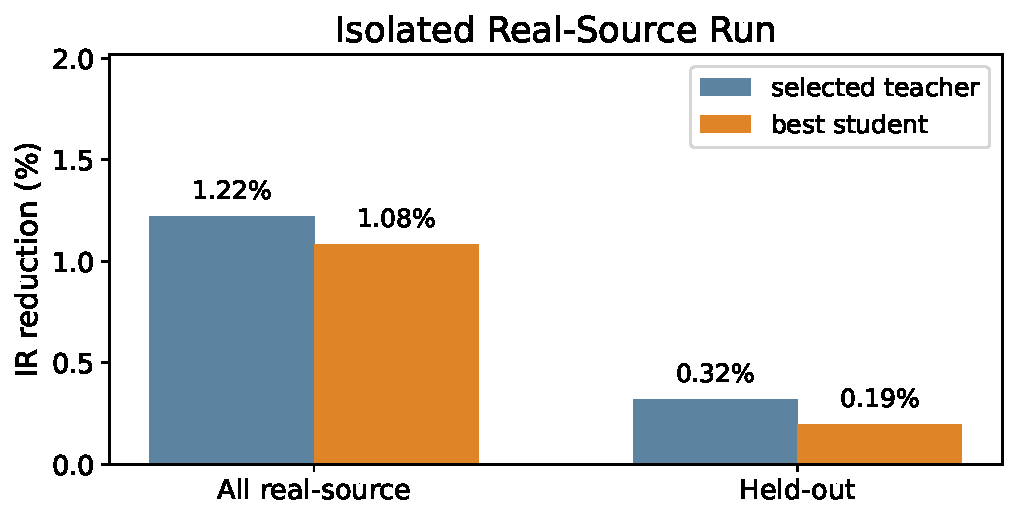
\includegraphics[width=0.56\linewidth]{../out/real_signal_run_all/summary_plot.pdf}
\caption{All-real-source isolated run. The experiment retrains and rewrites only
real-source modules; the plot visualizes the same reductions as the table.}
\label{tab:real-signal-all}
\end{table}

Positive reductions mean smaller rewritten IR than never-inline. The best
held-out student is \texttt{deep\_forest}, with 1559.62 average IR instructions,
a 0.61\% reduction, and a 7.58-instruction gap to the selected teacher. On the
full artifact set, \texttt{conservative\_forest} is best, reducing all modules
by 1.18\%. The held-out reductions remain small because many real-source modules
leave little profitable local inlining margin and because features are not
recomputed after each accepted rewrite.

Table~\ref{tab:llvm-oz-comparison} frames the learned policies as prototype
results rather than production replacements. On held-out rewritten objects,
\texttt{deep\_forest} reduces average \texttt{.text} from 5755.23 to 5705.23
bytes, but LLVM \texttt{-Oz} remains the much stronger native-size baseline.

A three-round BC-Max-style check also fed the previous best student back into
the candidate pool. The selected-policy reference stayed at 1.10\% held-out IR
reduction, and the best student stayed \texttt{deep\_forest} at 0.61\%, so the
small policy pool plateaued.

% =========================================================
% CHAPTER 9
% =========================================================

\chapter{Limitations}
\label{chap:limitations}

\begin{itemize}
\setlength{\itemsep}{2pt}
  \item \textbf{Dataset scale.} One of the most important limitations is the
  scale of the
  dataset. The run uses 163 compiled C/C++ files and 10394 call-site samples,
  including 76 public-source files. Broader transfer would still require larger
  benchmark families such as SPEC, cBench/MiBench, SQLite builds, and wider
  LLVM test-suite subsets.
  \item \textbf{Held-out scope.} The hold-out split has 1385 samples from 26
  unseen modules, but all modules still come from the same source snapshot and
  generator regime. A stronger future test would use modules from more clearly
  different sources.
  \item \textbf{Rewrite approximation.} Features are extracted only once in the
  main run, selected
  callees are cloned and marked \texttt{alwaysinline}, and LLVM \texttt{opt}
  performs the actual inlining. A fuller system would recompute features after
  each accepted rewrite, closer to LLVM's online inliner.
  \item \textbf{Metric scope.} Rewritten LLVM IR instruction count is the
  primary reward. Native \texttt{.text} and object-file size remain secondary;
  linked executable size and runtime are outside the current evaluation.
  \item \textbf{Teacher and MLGO scope.} BC-Max can only select among available
  candidate policies. The teachers are inspectable proxies rather than
  production inliner policies, and full MLGO reproduction would require deeper
  LLVM integration and a much larger corpus.
  \item \textbf{Iterative scope.} The added three-round BC-Max-style check feeds
  back the best student as a new measured policy, but it does not include the
  uncertainty-based trajectory exploration used in larger BC-Max systems.
  \item \textbf{Generated-data filtering.} A future generator could add a
  discriminator that rejects near-duplicate modules and keeps rarer inlining
  patterns before training.
\end{itemize}

% =========================================================
% CHAPTER 10
% =========================================================

\chapter{Conclusions}

The purpose of this thesis was to study how compiler inlining can be optimized
using offline methods for learning policies, and to implement a reproducible
end-to-end pipeline that works with LLVM IR. The reported run compiles 163 C/C++
sources, evaluates 150 modules with local call sites, evaluates 16 teacher-role
heuristics, trains 7 students, and applies learned decisions back to LLVM IR
through a call-site-level rewrite.

The main held-out result is measured on a source-level mix of DCMTK, generated
modules, and 76 public C/C++ source files. On the 26 held-out modules, the
selected-teacher reference reduces average rewritten LLVM IR instruction count
from 1569.23 to 1552.04, a 1.10\% reduction relative to the never-inline
teacher. When it comes to students, the best held-out model by IR size is
\texttt{deep\_forest}, which reaches 1559.62 instructions on average, a 0.61\%
reduction. On the full artifact set, \texttt{conservative\_forest} reaches
1961.94 instructions and reduces rewritten IR by 1.18\%.

As shown before the conclusion, LLVM \texttt{-Oz} is much stronger on the
standalone C/C++ files: relative to \texttt{no\_inline\_Oz}, it reduces native
\texttt{.text} size by 14.91\% and object-file size by 28.76\%. The learned
policies therefore demonstrate the workflow and formulation, not a
production-ready replacement for LLVM's full size pipeline.

The major contribution of this thesis is methodological: it connects source
collection, LLVM IR generation, feature extraction, teacher evaluation,
behavior-cloning dataset construction, student training, rewrite application,
and artifact-level measurement in one reproducible workflow. Stronger results
would require integration into LLVM's actual inliner, larger real benchmark
suites, stronger teacher policies, and final linked-binary measurements.

\appendix

\chapter{Additional Diagnostics}
\label{app:additional-diagnostics}

The generated \texttt{out/} directory contains the full JSON outputs used for
inspection. Figures~\ref{fig:appendix-teachers}
to~\ref{fig:appendix-decisions} keep the main diagnostics in portrait layout,
with readable labels and values.

\begin{figure}[H]
\centering
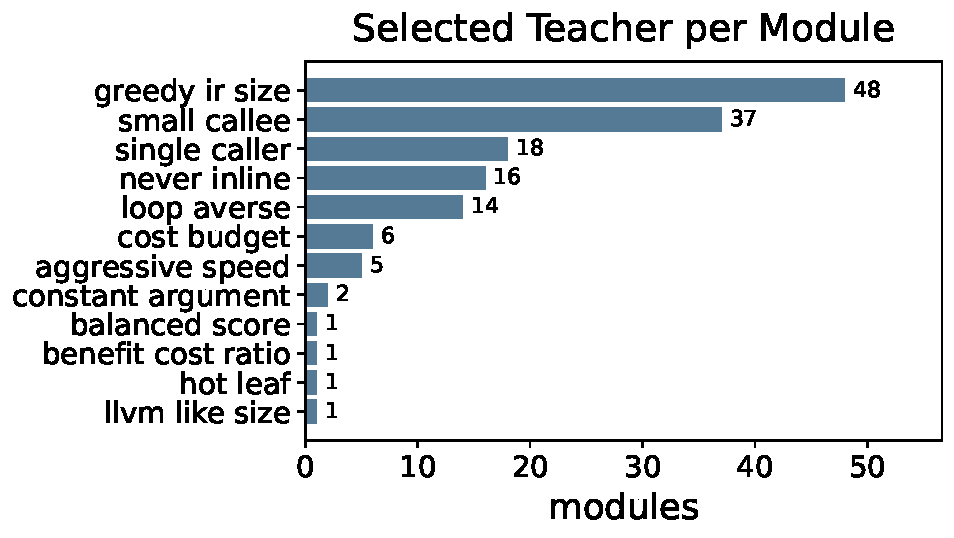
\includegraphics[width=0.74\linewidth,height=0.25\textheight,keepaspectratio]{selected_teacher_distribution.pdf}
\caption{Selected teacher distribution by module.}
\label{fig:appendix-teachers}
\end{figure}

\vspace{-0.6em}
\begin{figure}[H]
\centering
\begin{minipage}[t]{0.46\linewidth}
\centering
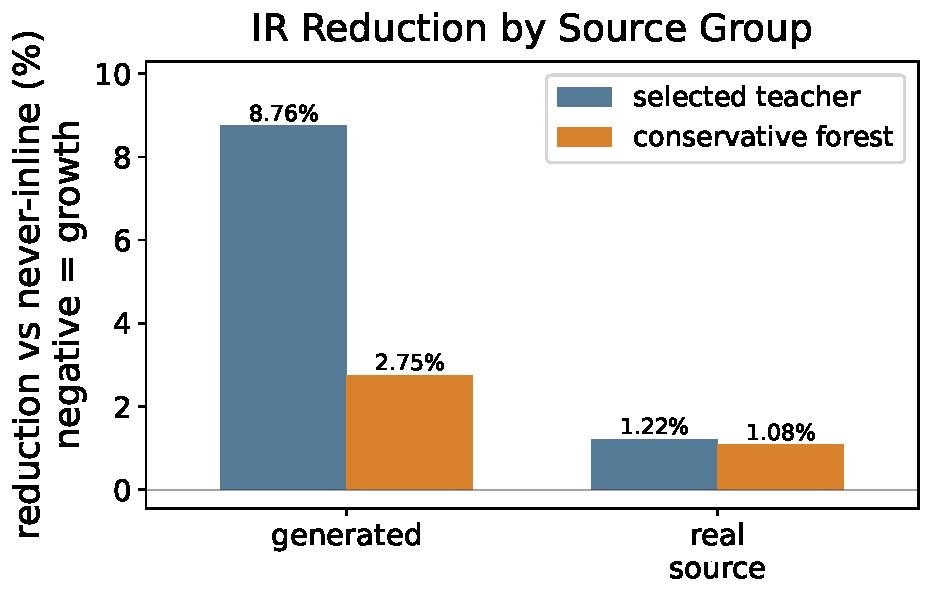
\includegraphics[width=\linewidth,height=0.20\textheight,keepaspectratio]{source_group_ir_reduction.pdf}
\caption{Teacher and student IR reduction by source group.}
\label{fig:appendix-source-groups}
\end{minipage}\hfill
\begin{minipage}[t]{0.50\linewidth}
\centering
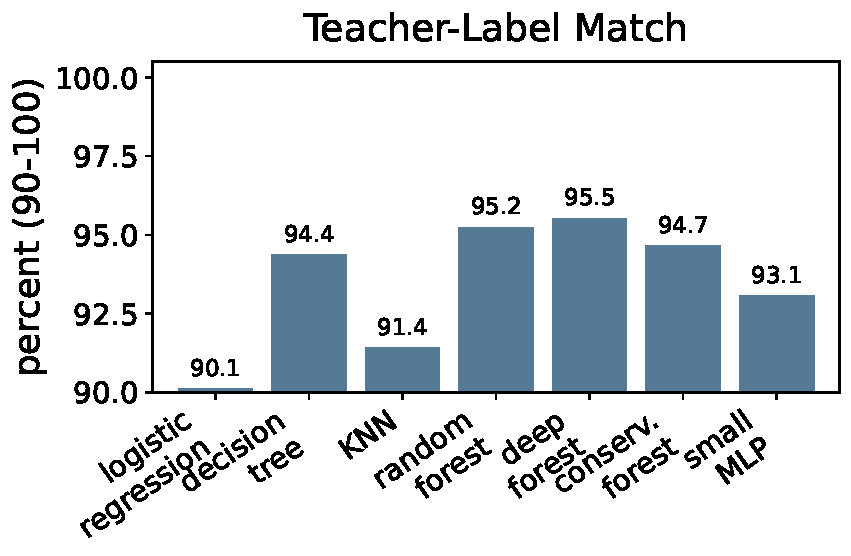
\includegraphics[width=\linewidth,height=0.22\textheight,keepaspectratio]{student_teacher_match.pdf}
\caption{Held-out teacher-label match for student models.}
\label{fig:appendix-student-match}
\end{minipage}
\end{figure}

\vspace{-0.6em}
\begin{figure}[H]
\centering
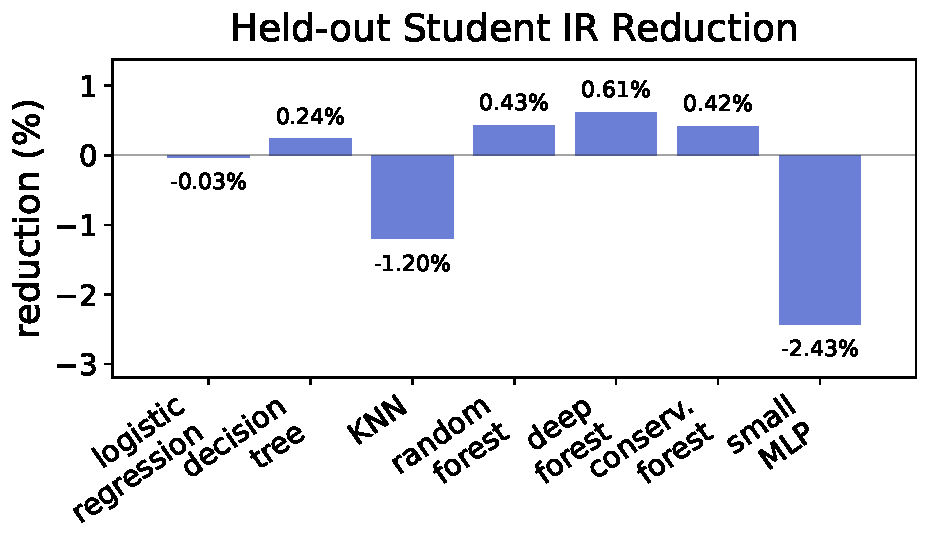
\includegraphics[width=0.86\linewidth,height=0.24\textheight,keepaspectratio]{student_ir_reduction.pdf}
\caption{Held-out student IR reduction.}
\label{fig:appendix-student-ir}
\end{figure}

\vspace{-0.6em}
\begin{figure}[H]
\centering
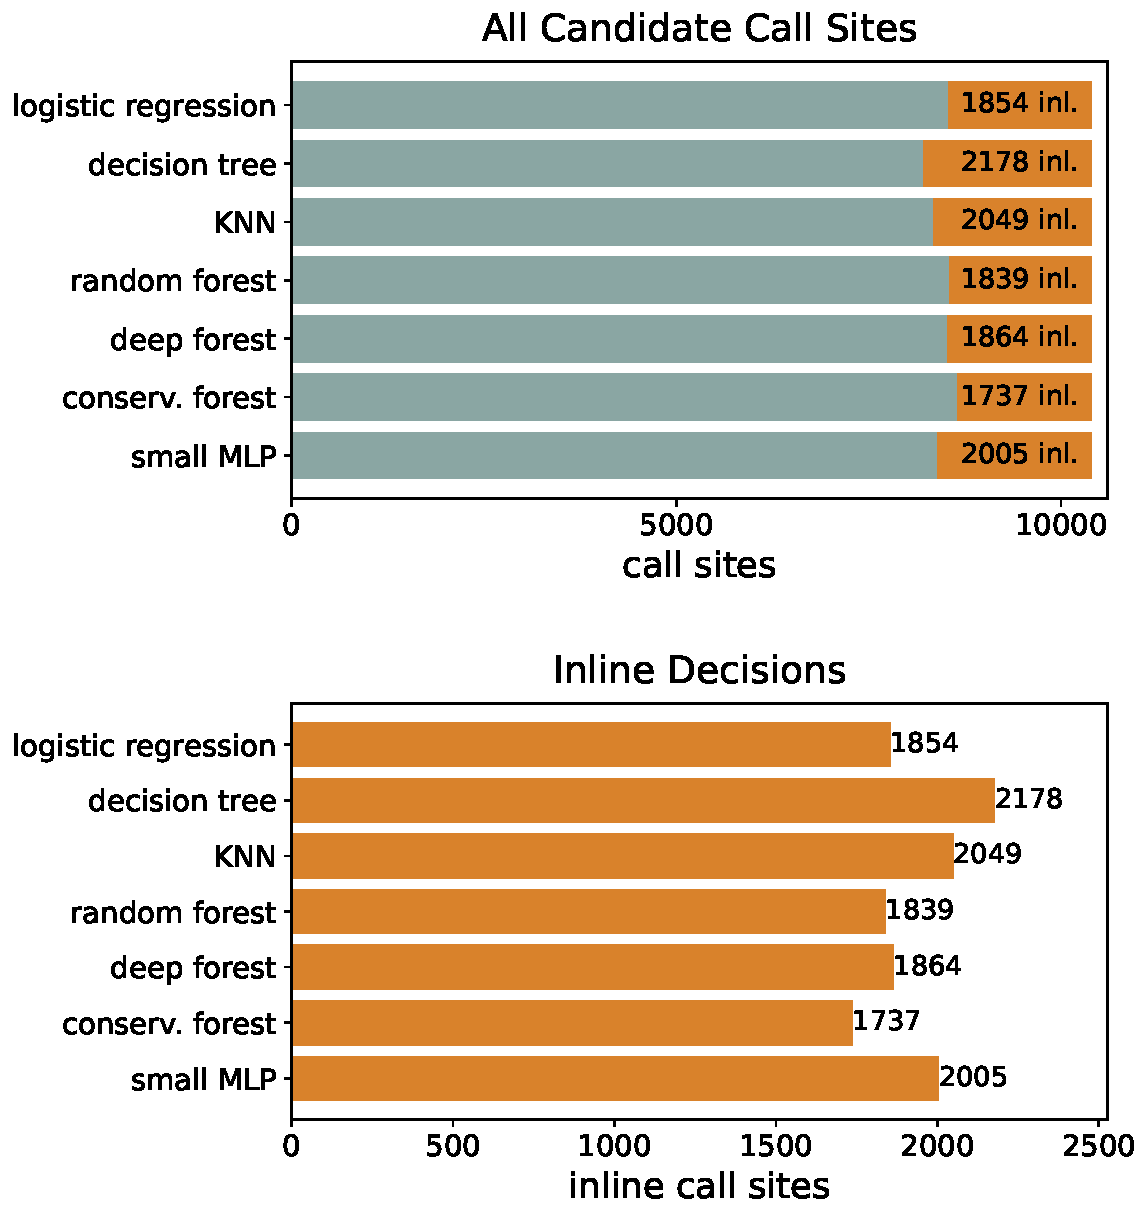
\includegraphics[width=\linewidth,height=0.42\textheight,keepaspectratio]{student_inline_decisions.pdf}
\caption{Student inline/no-inline decisions across candidate call sites.}
\label{fig:appendix-decisions}
\end{figure}

\begingroup
\tiny
\sloppy
\setlength{\bibitemsep}{0pt}
\setlength{\bibparsep}{0pt}
\setlength{\bibhang}{0pt}
\printbibliography[heading=bibintoc,title={Bibliography}]
\endgroup

\end{document}
